\documentclass[12pt,a4paper]{article}

% Packages
\usepackage[a4paper,top=2.5cm,bottom=2.5cm,left=2.5cm,right=2.5cm]{geometry}
\usepackage{graphicx}
\usepackage{array}
\usepackage{float}
\usepackage{setspace}
\usepackage{longtable}
\usepackage{xurl}
\usepackage[hidelinks]{hyperref}
\usepackage{caption}
\usepackage{needspace}
\usepackage{booktabs}
\usepackage{amsmath}
\usepackage{microtype}
\usepackage{titlesec}
\usepackage{flushend}
\DeclareCaptionFont{reportcaption}{\fontsize{9.5}{11}\selectfont}

% Global settings
\setstretch{1.08}
\setlength{\textfloatsep}{8pt plus 2pt minus 2pt}
\setlength{\intextsep}{8pt plus 2pt minus 2pt}
\setlength{\abovecaptionskip}{4pt}
\setlength{\belowcaptionskip}{2pt}
\setlength{\columnsep}{0.7cm}
\setlength{\emergencystretch}{1.5em}
\setlength{\Urlmuskip}{0mu plus 1mu}
\graphicspath{{./}{resultImage/}{image/}}
\newcommand{\sectionbreakguard}{\Needspace{8\baselineskip}}
\newcommand{\subsectionbreakguard}{\Needspace{7\baselineskip}}

% Centered column helper
\newcolumntype{C}[1]{>{\centering\arraybackslash}p{#1}}

% Document
\begin{document}
\hypersetup{pageanchor=false}

\begin{titlepage}
\centering

% Logos
\begin{minipage}[c]{0.44\textwidth}
  \raggedright
  
\includegraphics[width=3cm]{image/ITC_Tran_Logo.png}
\end{minipage}%
\hfill%
\begin{minipage}[c]{0.44\textwidth}
  \raggedleft
  
\includegraphics[width=3cm]{image/AMS-Logo.jpg}
\end{minipage}

\vspace{0.5cm}
\noindent\rule{\linewidth}{0.8pt}
\vspace{0.3cm}

% Institution
{\Large\bfseries INSTITUTE OF TECHNOLOGY OF CAMBODIA\par}

\vspace{0.25cm}

{\large\bfseries Department of Applied Mathematics and Statistics\par}

\vspace{0.2cm}
\noindent\rule{\linewidth}{0.4pt}
\vspace{1.2cm}

% Course
{\large\bfseries Probabilistic Graphical Models\par}

\vspace{0.3cm}

{\normalsize I4-AMS-DAS-A \quad (2025--2026)\par}

\vspace{1.5cm}

% Project title
{\LARGE\bfseries Building a Robust Part-of-Speech Tagger using Hidden Markov Model\par}

\vspace{1.8cm}

% Team table
{\large\bfseries Team 3\par}
\vspace{0.5cm}

\begin{minipage}{13.6cm}
\centering
\renewcommand{\arraystretch}{1.4}
\begin{tabular}{>{\raggedright\arraybackslash}p{6.5cm} C{3.8cm} C{2cm}}
  \toprule
  \textbf{Name of Student} & \textbf{Student ID} & \textbf{Score} \\
  \midrule
  1.\enspace HEAM VISAL        & e20221349           & \dots \\
  2.\enspace MON Sreylin       & e20221701           & \dots \\
  3.\enspace CHOUB Botumraksa  & e20221709           & \dots \\
  4.\enspace CHIV Mengchou     & e20221028           & \dots \\
  \bottomrule
\end{tabular}
\end{minipage}

\vfill

% Footer
\noindent\rule{\linewidth}{0.4pt}\\[6pt]
\begin{minipage}[t]{13.6cm}
  \raggedright
  \begin{tabular}{@{}l@{\enspace}l@{}}
    \textbf{Lecturer:} & Mr. PHOK Ponna \\
  \end{tabular}
\end{minipage}

\end{titlepage}

\clearpage
\hypersetup{pageanchor=true}

\pagenumbering{roman}
\tableofcontents
\clearpage
\pagenumbering{arabic}

% Compact two-column report style (applied only after the contents page)
\newgeometry{top=1.8cm,bottom=1.8cm,left=1.8cm,right=1.8cm}
\setlength{\columnsep}{0.82cm}
\setstretch{1.0}
\fontsize{11}{13}\selectfont
\captionsetup{font=reportcaption,skip=3pt}
\titleformat{\section}{\sffamily\bfseries\fontsize{12}{13.5}\selectfont}{\thesection}{0.55em}{\MakeUppercase}
\titleformat{name=\section,numberless}{\sffamily\bfseries\fontsize{12}{13.5}\selectfont}{}{0pt}{\MakeUppercase}
\titleformat{\subsection}{\sffamily\bfseries\fontsize{11}{13}\selectfont}{\thesubsection}{0.55em}{}
\titlespacing*{\section}{0pt}{1.25ex plus 0.4ex minus 0.2ex}{0.55ex}
\titlespacing*{\subsection}{0pt}{1.0ex plus 0.3ex minus 0.2ex}{0.4ex}
\setlength{\textfloatsep}{7pt plus 2pt minus 2pt}
\setlength{\dbltextfloatsep}{5.5pt plus 2pt minus 1.5pt}
\setlength{\floatsep}{6pt plus 2pt minus 2pt}
\setlength{\intextsep}{6pt plus 2pt minus 2pt}
\twocolumn

\sectionbreakguard
\section{Abstract}

This report presents a Part-of-Speech (POS) tagger based on a Hidden Markov Model
(HMM). The system was implemented from scratch and evaluated on the Brown Corpus
from NLTK using the universal POS tagset. The task is to assign the most likely
POS tag to each word in a sentence. The dataset contains 57,340 sentences and was
divided into 80\% training data and 20\% testing data. The HMM parameters were
estimated using Maximum Likelihood Estimation from frequency counts. To handle
unseen words, Laplace smoothing with $\alpha = 1.0$ and a special
\texttt{\textless OOV\textgreater} token were used. The Viterbi algorithm was
implemented in log-space to avoid numerical underflow. On the test set, the model
tagged 217,777 out of 232,177 words correctly, giving an accuracy of 93.8\%.
The results show that a compact statistical sequence model can recover most tag
assignments from local sequential regularities. The remaining errors are
concentrated around lexical ambiguity, sparse training evidence, and unseen
words, which are limitations expected from the model assumptions and the chosen
emission representation.

\sectionbreakguard
\section{Introduction}

Part-of-Speech tagging is a basic task in Natural Language Processing (NLP). It
assigns a grammatical category, such as noun, verb, adjective, or adposition, to
each word in a sentence. POS tagging is useful because it provides syntactic
information for many later NLP tasks, including parsing, information extraction,
machine translation, and text analysis.

This mini project builds a POS tagger using a Hidden Markov Model. An HMM is a
probabilistic model for sequence data. In this task, the observed sequence is the
sentence, and the hidden sequence is the POS tag sequence. The model assumes that
each tag depends mainly on the previous tag, and that each word is generated from
its tag.

The project uses the Brown Corpus from NLTK with the universal POS tagset. The
universal tagset reduces the original detailed tag labels into 12 general POS
tags. This makes the task simpler and allows the model to focus on common
grammatical categories. The main objective is to train the HMM from the training
sentences and use it to predict POS tags for unseen test sentences.

The work follows a complete supervised sequence-labeling pipeline. Tagged
sentences provide the counts needed to estimate the model, a held-out portion of
the corpus measures generalization, and Viterbi decoding converts the learned
probabilities into one globally consistent tag sequence per sentence. This is
important because selecting the most frequent tag for each word independently
would ignore the way grammatical categories tend to follow one another.

The HMM also provides an interpretable baseline. Its initial, transition, and
emission components have direct probabilistic meanings, so a prediction can be
related to sentence-start patterns, neighboring tags, and word--tag evidence.
At the same time, the model deliberately uses limited context. Evaluating it
therefore shows both how much can be learned from first-order dependencies and
where richer lexical or contextual information would be needed.

\sectionbreakguard
\section{Methodology}

\subsectionbreakguard
\subsection{Dataset and Tagset}

The dataset used in this project is the Brown Corpus provided by NLTK. The
corpus was loaded with the universal POS tagset. In total, the dataset contains
57,340 tagged sentences. The data was split into 45,872 training sentences and
11,468 testing sentences, following an 80\%--20\% split. The vocabulary size in
the training data is 45,153, and the number of POS tags is 12.

The sentence list was shuffled with random seed 42 before the split, making the
experiment reproducible while keeping complete sentences together. No test
sentence contributes counts to parameter estimation. This separation matters:
the reported accuracy measures predictions on held-out sentences rather than
the model's ability to reproduce the observations from which its probabilities
were calculated. Words are normalized to lowercase for vocabulary lookup and
emission counting, so capitalization variants share the same lexical evidence.

\begin{figure}[!htbp]
    \centering
    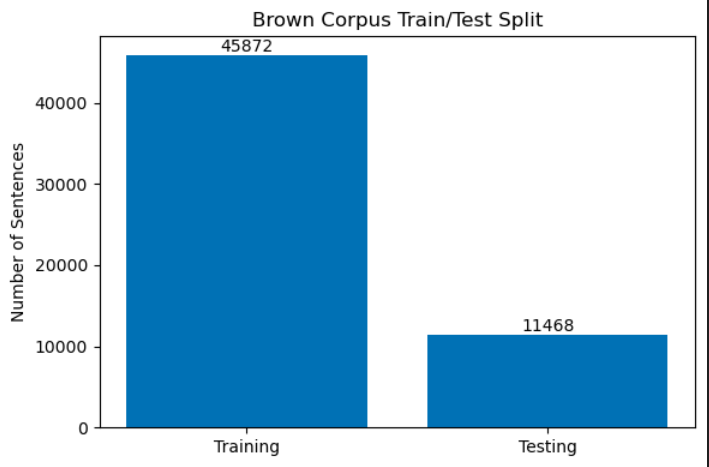
\includegraphics[width=0.98\linewidth, trim=0 0 14pt 0, clip]{resultImage/Dataset-split-result.png}
    \caption{Dataset split between training and testing sentences.}
    \label{fig:dataset-split}
\end{figure}

\subsectionbreakguard
\subsection{Hidden Markov Model}

The POS tagging problem is modeled as a sequence prediction problem. Given a
sentence $w_1, w_2, \ldots, w_n$, the goal is to find the most likely tag sequence
$t_1, t_2, \ldots, t_n$. The HMM represents the joint probability of the tag and
word sequence as:

\begin{equation}
\begin{aligned}
&P(t_1, \ldots, t_n, w_1, \ldots, w_n) \\
&= \pi(t_1) B_{t_1}(w_1)
\prod_{i=2}^{n} A_{t_{i-1},t_i} B_{t_i}(w_i)
\end{aligned}
\end{equation}

In this formula, $\pi$ is the initial probability, $A$ is the transition
probability matrix, and $B$ is the emission probability matrix. These parameters
are estimated from the training data.

The factorization makes two simplifying assumptions. First, the tag at position
$i$ is conditioned on the tag at position $i-1$ rather than on the entire tag
history. Second, once the current tag is known, the observed word is treated as
independent of the other words and tags. Under these assumptions, $\pi(t_1)$
scores a possible sentence opening, each $A_{t_{i-1},t_i}$ scores a local tag
change, and each $B_{t_i}(w_i)$ scores the compatibility of a word with its tag.
Multiplying the factors assigns a score to a complete word--tag sequence.

Although the hidden tags are available during supervised training, they are not
available when a new sentence is decoded. At prediction time the words are the
observations and the POS labels are hidden states that must be inferred jointly.
This separation between observed words and latent test-time states is the reason
the tagging task fits the HMM formulation.

\subsectionbreakguard
\subsection{Parameter Estimation}

The model parameters were estimated using Maximum Likelihood Estimation based on
frequency counts. The initial probability estimates how likely a tag is to start
a sentence:

\begin{equation}
\pi(t) = \frac{\text{Count}(t \text{ starts a sentence})}
{\text{Total sentences}}
\end{equation}

The transition probability estimates how likely tag $j$ is to follow tag $i$:

\begin{equation}
A(i,j) = \frac{\text{Count}(\text{tag}_i \text{ followed by } \text{tag}_j)}
{\text{Count}(\text{tag}_i)}
\end{equation}

The emission probability estimates how likely word $w$ is generated by tag $t$.
Laplace smoothing was used to reduce zero-probability problems:

\begin{equation}
B(t,w) = \frac{\text{Count}(w \text{ emitted by } t) + \alpha}
{\text{Count}(t) + \alpha (|V| + 1)}
\end{equation}

Here, $V$ is defined as the set of distinct normalized words observed in the
training data; it excludes the special \texttt{\textless OOV\textgreater}
token. The additional 1 in $|V|+1$ accounts for that OOV outcome. In this
project, $\alpha = 1.0$. During testing, words not found in $V$ were mapped to
the OOV token. Its emission probability for tag $t$ is therefore

\begin{equation}
B(t,\text{OOV}) = \frac{\alpha}
{\text{Count}(t) + \alpha (|V| + 1)}.
\end{equation}

The three estimates summarize different count tables. Initial counts are
collected only from the first token of each training sentence. Transition counts
are collected from adjacent tag pairs within a sentence, so sentence boundaries
do not create artificial transitions. Emission counts are collected from
normalized word--tag pairs. Dividing each count by its appropriate total turns
the table into a conditional probability distribution.

Laplace smoothing is applied to emissions over the $|V|$ observed training
words plus the one additional OOV outcome. It gives every
word--tag combination a non-zero probability, while combinations observed many
times still receive greater probability mass. The initial and transition
distributions are estimated without Laplace smoothing in this implementation.
When decoding, a small numerical constant is added before taking logarithms so
that a zero estimate does not cause an undefined computation. This numerical
safeguard should not be confused with re-estimating those distributions with
smoothing.

\subsectionbreakguard
\subsection{Decoding with Viterbi Algorithm}

After estimating the HMM parameters, the Viterbi algorithm was used to find the
best tag sequence for each test sentence. The algorithm uses dynamic programming
to avoid checking all possible tag sequences directly. Since multiplying many
small probabilities can cause computational underflow, the implementation uses
log-space. For a candidate tag $j$, initialization combines the sentence-start
and first-word probabilities:

\begin{equation}
\log v_1(j) = \log \pi(j) + \log B(j,w_1).
\end{equation}

For positions $t=2,\ldots,n$, the recurrence keeps the best score ending in
$j$:

\begin{equation}
\begin{aligned}
\log v_t(j) ={} &\max_i \left[\log v_{t-1}(i)
                    + \log A(i,j)\right] \\
                  &+ \log B(j,w_t).
\end{aligned}
\end{equation}

At the same time, the backpointer records which previous tag attained that
maximum:

\begin{equation}
\psi_t(j) = \underset{i}{\arg\max}\,
\left[\log v_{t-1}(i) + \log A(i,j)\right].
\end{equation}

The best final tag is selected from the last Viterbi column, after which the
stored backpointers reconstruct the path in reverse:

\begin{equation}
\begin{aligned}
\hat{t}_n &= \underset{j}{\arg\max}\,\log v_n(j), \\
\hat{t}_{t-1} &= \psi_t(\hat{t}_t),
\quad t=n,n-1,\ldots,2.
\end{aligned}
\end{equation}

The model stores the best previous tag for each current tag and then performs
backtracking to recover the predicted tag sequence.

Initialization combines the initial probability of each possible first tag with
the first word's emission probability. For every later position, the recurrence
examines all previous tags and retains only the highest-scoring path ending in
each current tag. After the final word, the best final state is selected and the
stored backpointers are followed in reverse. With $n$ words and $T$ tags, this
requires $O(nT^2)$ score comparisons instead of enumerating $T^n$ complete tag
sequences.

Log-space changes products into sums and preserves the ordering of path
probabilities because the logarithm is monotonic. It therefore produces the same
maximum-probability path as direct multiplication, subject to numerical
precision, but avoids the rapid underflow caused by multiplying many values
smaller than one.

\sectionbreakguard
\section{Results and Evaluation}

\subsectionbreakguard
\subsection{Evaluation Metric}

The model was evaluated using word-level accuracy. Accuracy measures the
proportion of test words whose predicted POS tag is equal to the true POS tag:

The evaluation iterates through every token in the 11,468 held-out sentences.
Each prediction is compared at the same sentence position with its corpus tag;
correct comparisons are summed and divided by the total number of test tokens.
This micro-averaged measure gives every word equal weight, regardless of its
sentence length or tag frequency. It is easy to interpret, but it does not show
whether performance is distributed uniformly across tags, known words, and OOV
words. The subsequent counts and error analysis provide that additional context.

\begin{equation}
\text{Accuracy} =
\frac{\text{Correctly tagged words}}{\text{Total test words}}
\end{equation}

\subsectionbreakguard
\subsection{Final Evaluation Summary}

Table~\ref{tab:summary} shows the final evaluation summary. The model achieved
93.8\% accuracy on 232,177 test words. Out of these words, 217,777 were tagged
correctly and 14,400 were tagged incorrectly.

The displayed percentage is rounded: the underlying evaluation counts are the
primary result and satisfy $217{,}777 + 14{,}400 = 232{,}177$. Thus, the summary
table and bar chart report the same evaluation from complementary views. The
training and testing sentence counts also agree with the dataset split in
Figure~\ref{fig:dataset-split}; they are included here to make the experimental
scale visible beside the final score.

\begin{table}[!htbp]
    \centering
    \fontsize{9.5}{11}\selectfont
    \begin{tabular}{@{}lr@{}}
        \toprule
        \textbf{Metric} & \textbf{Value} \\
        \midrule
        Training sentences & 45,872 \\
        Testing sentences & 11,468 \\
        Vocabulary size & 45,153 \\
        POS tags & 12 \\
        Total test words & 232,177 \\
        Correct words & 217,777 \\
        Wrong words & 14,400 \\
        Accuracy & 93.8\% \\
        OOV words & 5,050 \\
        OOV rate & 2.18\% \\
        \bottomrule
    \end{tabular}
    \caption{Final Evaluation Summary}
    \label{tab:summary}
\end{table}

\begin{figure}[!htbp]
    \centering
    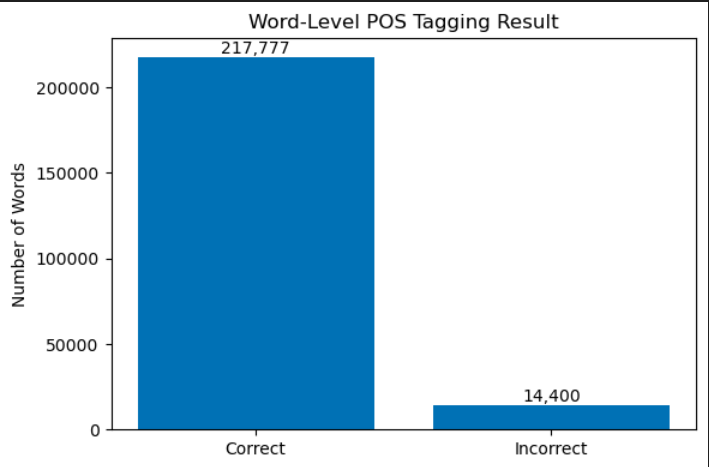
\includegraphics[width=\linewidth, trim=0 0 13pt 0, clip]{resultImage/Final-accuracy-result-with-numbers-on-bars.png}
    \caption{Word-level POS tagging result on the test set.}
    \label{fig:word-result}
\end{figure}

\subsectionbreakguard
\subsection{OOV Analysis}

The test set contains 5,050 OOV words, giving an OOV rate of 2.18\%. OOV words
are words that do not appear in the training vocabulary. The model handles these
words using Laplace smoothing and the \texttt{\textless OOV\textgreater} token.
This allows the model to assign non-zero emission probabilities to unseen words.
However, OOV words are still difficult because the model has no direct training
evidence for their most likely tags.

The 5,050 OOV tokens are counted at test time by checking normalized words
against the 45,153-word training vocabulary. The remaining 227,127 test tokens
are known to the model. Therefore, the OOV analysis measures vocabulary coverage
rather than a separate test subset, and the OOV and known counts together equal
the total number of evaluated words.

For an unseen word, every tag receives its tag-specific smoothed OOV emission
probability. The decoder must then rely more heavily on the initial probability
and surrounding transition patterns because no observed word--tag count
identifies the word directly. Smoothing keeps decoding possible, but it does not
use spelling, prefixes, suffixes, or other morphological cues that might
separate likely nouns, verbs, and adjectives.

\begin{figure}[!htbp]
    \centering
    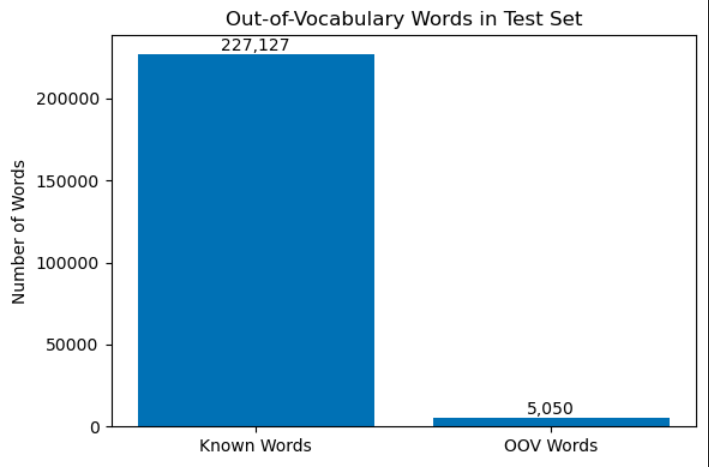
\includegraphics[width=0.95\columnwidth, trim=0 0 13pt 0, clip]{resultImage/OOV-analysis-result-with-numbers-on-bars.png}
    \caption{OOV word analysis on the test set.}
    \label{fig:oov-analysis}
\end{figure}

\begin{figure*}[!t]
    \centering
    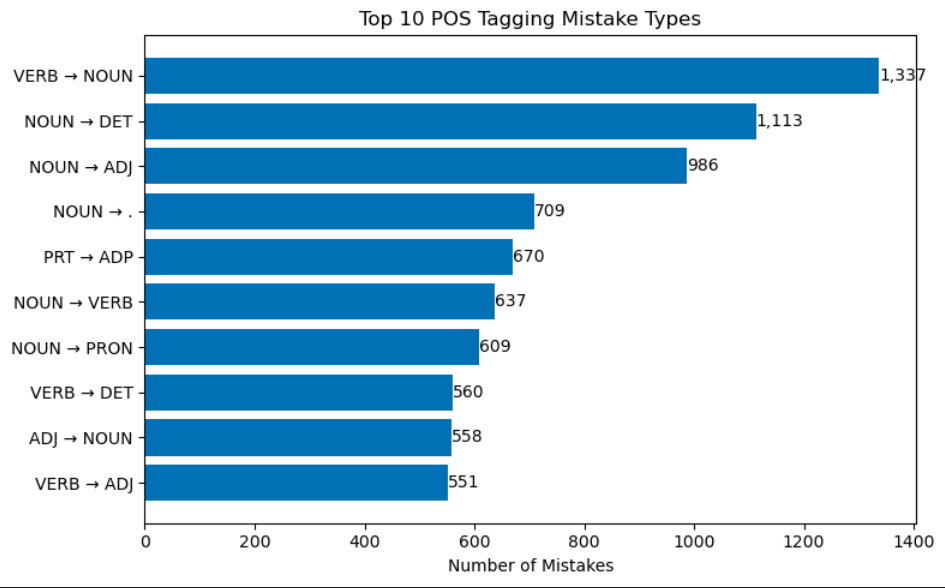
\includegraphics[width=0.78\textwidth]{resultImage/Top-10-mistake-types-with-numbers-on-bars.png}
    \caption{Top 10 POS tagging mistake types.}
    \label{fig:top-mistakes}
\end{figure*}

\sectionbreakguard
\section{Error Analysis}

The model made 14,400 word-level mistakes on the test set. Many mistakes happen
because some English words are ambiguous. A word can have different POS tags
depending on how it is used in a sentence. For example, ``average'' can be a
noun, adjective, or verb depending on context. Similarly, ``offer'' can be a noun
or a verb.

Table~\ref{tab:error-examples} shows selected failed examples from the test
sentences.

The aggregate mistake chart in Figure~\ref{fig:top-mistakes} shows that errors
are not evenly distributed. The largest direction is VERB predicted as NOUN
(1,337 cases), followed by NOUN predicted as DET (1,113) and NOUN predicted as
ADJ (986). Direction matters: NOUN predicted as VERB has 637 cases and is a
different error category from VERB predicted as NOUN. Together, the ten displayed
categories contain 7,730 of the 14,400 wrong predictions, so a substantial
remainder is spread across less frequent confusion types.

\begin{table*}[!t]
    \centering
    \fontsize{9.5}{11}\selectfont
    \begin{tabular}{p{0.40\textwidth}p{0.14\textwidth}p{0.14\textwidth}p{0.20\textwidth}}
        \toprule
        \textbf{Sentence} & \textbf{Word} & \textbf{True Tag} & \textbf{Predicted Tag} \\
        \midrule
        With tips, the girls average between \$150 and \$200 a week, depending on basic salary.
        & average & VERB & NOUN \\
        & \$200 & NOUN & ADP \\
        & depending & ADP & VERB \\
        \midrule
        It was a very tempting offer.
        & very & ADV & ADJ \\
        & tempting & VERB & NOUN \\
        & offer & NOUN & VERB \\
        \midrule
        He saw the surprise in her face, and laughed as though it were the funniest expression he had ever seen.
        & as & ADP & ADV \\
        \bottomrule
    \end{tabular}
    \caption{Error Analysis Examples}
    \label{tab:error-examples}
\end{table*}

These failures directly reflect the first-order Markov assumption, under which
each tag depends only on the preceding tag rather than the full sentence context.
In ``With tips, the girls average\ldots'', ``average'' is ambiguous among NOUN,
ADJ, and VERB. Local tag transitions favored NOUN, and that wrong path also
affected nearby predictions such as ``\$200'' and ``depending.'' The words ``tempting'' and ``offer'' in ``It was a very tempting offer.''
are lexically ambiguous.
Relying only on local transition and emission probabilities, the HMM selected an
incorrect sequence without understanding the sentence meaning. Finally, in ``He
saw the surprise\ldots laughed as though\ldots'', ``as'' can be ADP or ADV.
Recognizing the construction ``as though'' requires longer context than this
first-order HMM represents.

Rare words and unseen words are also challenging. Laplace smoothing helps by
preventing zero probabilities, but it cannot fully replace real evidence from
training data. Therefore, OOV words can still receive incorrect tags, especially
when they appear in unusual contexts.

The examples also illustrate why a single wrong decision can affect nearby
positions. Viterbi chooses a complete path, and a locally attractive transition
can change the best continuation for later words. Consequently, the rows in
Table~\ref{tab:error-examples} should be read as outcomes of sequence decoding,
not as independent word classifications. The table is illustrative; the overall
counts and top mistake types summarize the complete test set.

\sectionbreakguard
\section{Conclusion}

This project implemented a POS tagger using a Hidden Markov Model trained on the
Brown Corpus with the universal POS tagset. The model estimated initial,
transition, and emission probabilities from frequency counts using Maximum
Likelihood Estimation. Laplace smoothing with $\alpha = 1.0$ and a
\texttt{\textless OOV\textgreater} token were used to handle unseen words. The
Viterbi algorithm was implemented in log-space to decode the most likely POS tag
sequence while avoiding computational underflow.

The final result shows that the HMM POS tagger achieved 93.8\% accuracy on the
test set, corresponding to 217,777 correct predictions among 232,177 words. The
result demonstrates that initial-tag tendencies, adjacent-tag transitions, and
word emissions capture enough regularity to label most tokens correctly. Because
the score is computed on the held-out 20\% split, it evaluates generalization to
sentences that did not provide the training counts.

The analysis also identifies clear boundaries of the approach. The test set
contains 5,050 OOV tokens, for which the model has no word-specific training
count, and the most frequent mistakes involve confusions among common grammatical
categories. The first-order state assumption represents only the previous tag,
while the emission model uses a normalized word identity without morphological
or semantic features. These design choices explain why smoothing prevents
failure on unseen input but cannot resolve every ambiguous use.

Future improvements should be evaluated with the same fixed split so that their
effect can be compared directly with this baseline. Candidate extensions include
suffix or other word-form features for unknown words, higher-order tag
dependencies for broader local context, and neural sequence models that learn
contextual representations. Such extensions add complexity, so the current HMM
remains useful as a transparent reference model whose probabilities, decoding
steps, and error counts can be inspected directly.

\sectionbreakguard
\begingroup
\fontsize{10}{12}\selectfont
\begin{thebibliography}{9}

\bibitem{nltkbook}
Steven Bird, Ewan Klein, and Edward Loper.
\textit{Natural Language Processing with Python: Analyzing Text with the Natural Language Toolkit}.
O'Reilly Media, 2009. Official online version available at
\url{https://www.nltk.org/book/}.

\bibitem{nltkcorpus}
NLTK Project.
\textit{NLTK Corpus Reader Documentation}.
Official documentation showing access to the Brown Corpus and the universal POS
tagset. Available at \url{https://www.nltk.org/howto/corpus.html}.

\bibitem{viterbi}
Andrew J. Viterbi.
Error bounds for convolutional codes and an asymptotically optimum decoding
algorithm.
\textit{IEEE Transactions on Information Theory}, 13(2):260--269, 1967.
DOI: \url{https://doi.org/10.1109/TIT.1967.1054010}.

\bibitem{rabiner}
Lawrence R. Rabiner.
A tutorial on hidden Markov models and selected applications in speech
recognition.
\textit{Proceedings of the IEEE}, 77(2):257--286, 1989.
DOI: \url{https://doi.org/10.1109/5.18626}.

\end{thebibliography}
\endgroup

\end{document}
